\documentclass[11pt, letterpaper, oneside]{article}
\usepackage{enumerate}
\usepackage{ calc }
\usepackage{ amssymb }
\usepackage{graphicx}

\begin{document}

\title{\textbf{CMCS 818J Project Final Report} \\ Implementing Streaming Authenticated Data Structures}
\author{Behzad Koosha, Christopher Imbriano}

\maketitle

\section{Abstract}

	While Infrastructure and Platform -as-a-Service products provide clients access to large amounts of computing power and storage capacity, the client must trust the provider with their computation.
	It may be the case that verifying, by replication of the computation, requires too many resources and is infeasible for the client.
	In this report we will discuss a scheme for computation verification in a streaming setting; that is, one in which a client and provider both witness a stream of data.
	In this setting the client is assumed to have limited resources in both storage and computational power, and must rely on the provider to serve as a database of sorts from which the client can query about the data stream.

	Shi and Papamanthou \cite{sads} proposed a scheme called Streaming Authenticated Data Structures which allows a client to verify the correctness and completeness of answers to queries given by an untrusted party.
	The scheme has been shown to be secure and efficient requiring no communication between the client and the provider during the streaming setting.
	The goal of this project is twofold: first, produce this data structure as a library primitive and second produce an application demonstrating the library.
	So far we have implemented this type of data structure as a Ruby library and written a script to demonstrate the basic properties second.
	We also outline improvements and tasks required to realize an application using the SADS primitive.


\section{Introduction}

	A verifiable computation (VC) is one in which computation can be performed by a server on behalf of a client where the server is an untrusted resource.
	In this scenario, the client usually cannot, or wishes not to, perform the entire computation themselves but requires a means of verifying the computation efficiently.
	The growth of outsourced computation in the form of cloud computing has attracted a strong interest in the VC problem.
	In the streaming setting, many solutions to this problem have been proposed but so far have required inefficient protocols requiring the client and server to communicate updates as each stream element arrives.
	This communication requirement is prohibitively expensive in certain streaming applications where elements arrive in rapid succession, or are continuous.

	The Streaming Authenticated Data Structure scheme (SADS) \cite{sads} does not require any interaction between the client and the server while the stream is observed.
	Three important properties are obtained using this scheme :
	\begin{enumerate}[a.]
		\item Independence of prover (server) and verifier (client) : the prover and the verifier can update internal state without interaction.
		\item Efficiency : SADS demonstrates an exponential improvement in server's running time for many common query types.
		\item Expressiveness : a wide range of queries such as (non-)membership, successor, range search and frequencies can be supported
	\end{enumerate}
	The ultimate goal of the proposed scheme is to implement the SADS scheme that enable the verification of computation performed by an untrusted resource.

	The rest of this paper is organized as follows.
	Section \ref{sec:tree} will discuss the key data structure use to achieve the SADS goals.
	Section \ref{sec:parts} will discuss the key components in the SADS scheme.
	Section \ref{sec:impl} will discuss details of our implementation and section \ref{sec:forward} will discuss preliminary measurements and outline future improvements.

\section{ Achieving Independence through \\ a Lattice-based Hash Tree }
\label{sec:tree}

	The core concept that enables the SADS scheme to satisfy its desired goals is a lattice-based hash tree, also known as a Merkle tree.
	In traditional Merkle trees a hash function, such as SHA-1, is used to compute the value of any internal node of the tree.
	SHA-1, and similar hashes, are not homomorphic hash functions; that is, the hash of the sum of two elements is not necessarily the sum of the hash of the individual elements.
	For example, suppose there is a hash $h(x, y)$, a homomorphic hash would satisfy the following relation:
	\begin{equation}
		h(x + y) = h(x) + h(y)
	\end{equation}
	The key to the SADS scheme is Merkle tree using a homomorphic hash function which allows each node in the tree to be represented as a sum of parts, including the root of the tree.

	The homomorphic hash function in the SADS scheme maps what are called \textit{labels} to \textit{digests}, where labels and digests are different representations of the same value for each node.
	As in a traditional Merkle tree, each internal node derives its value from the hash of its children.
	In this case, a parent's digest is exactly the hash of its children's labels.
	This concept is depicted in figure \ref{fig:labels-and-digests}.
	Each node in the tree has a label $\lambda$ and a digest \textit{d}.

        \begin{figure}[h]
        \centering
        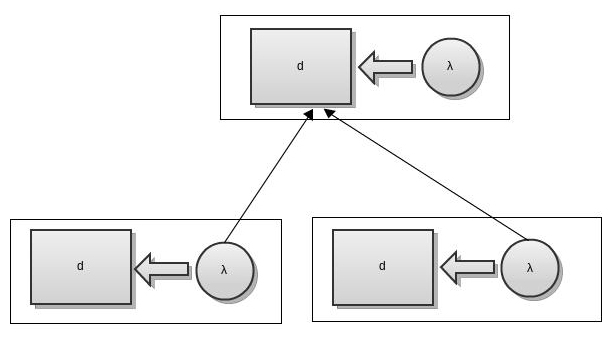
\includegraphics[width=100mm]{./images/label_digest.jpg}
        \caption[]{Labels and Digests}
        \label{fig:labels-and-digests}
        \end{figure}

	The crucial property of the hash function in the SADS scheme, which will only be briefly described here, allows every node in the tree to be represented by a sum of representations of its children.
	Each of those children can be represented as a sum of their children and so on.
	In this way, even the root of the tree can be represented by a sum of representations of the leaves of the tree.
	The representation being alluded to is called a \textit{partial digest} and is calculated for a particular node \textit{with respect to} some descendant in that nodes subtree.

	For example, suppose a tree is to represent a set of elements drawn from a universe of integers in the range $0 \leq x \leq 7$.
	To represent the root of such a tree in which the set of nodes \{1, 4, 6, 7\} are present, then digest of the root of the tree can be expressed as a sum of partial digests of the root, with respect to the present elements.
	That is,
	\begin{equation}
		\textit{D}(root, 1)+\textit{D}(root, 4)+\textit{D}(root, 6)+\textit{D}(root, 7)
	\end{equation} 
	where $\textit{D}(root, x)$ is the partial digest of the root with respect to x.
	This type of hash function is what allows the client (verifier) to maintain a correct running digest of all the stream elements seen, regardless of how large the tree is or how many stream elements have been witnessed.

	For the readers knowledge, we describe the hash function, but will not go into detail.  The proof of its security and correctness properties can be found in \cite{sads}.
	The hash function is given by,

	\begin{equation}
		h(x,y)= \textbf{L} x + \textbf{R}y
	\end{equation}
	where $x, y$ are labels of nodes, represented as vectors, $\textbf{L}, \textbf{R}$ are matrices performing the role of a public key in the scheme and $h(x,y)$ is a digest also represented as a vector.

\section{ Participants }
\label{sec:parts}

	\subsection{ Verifier and Prover }

		As mentioned previously, the verifier (or client) is a low resource computational device.
		It is expected that the verifier will not have sufficient storage capacity to store every element of a stream witnessed and therefore cannot correctly answer queries over the data stream elements.
		To accomplish these tasks, the verifier will rely on a more powerful device.
		The verifier will however have the means to store a digest, a small representation of all the elements it has seen.
		It will also be able to efficiently update its local state so as to not disrupt viewing elements of the stream.
		The verifier's only operation during the streaming phase will be to update its local state with some representation of each element of the stream, specifically a partial digest.

		The prover (server) on the other hand will act as a database.
		Internally, the prover maintains a representation of the stream elements witnessed such that it can answer queries from the verifier.
		That internal representation is the hash tree mentioned earlier which allows for a node to be update without rehashing its children.
		The verifier will exploit this property to maintain and update the root digest of the tree without communication with the prover.

		\subsection{ Query Proof }

		During or after the streaming phase, the verifier may wish to issue queries to the prover (server) of the form (non-)membership, successor, range, frequency etc. 
		The prover is expected to provide an answer to the query as well as a proof that can be efficiently verified by the verifier.
		Figure \ref{fig:proof} gives a visual representation of a membership proof for the green leaf node.
		The whole set of green nodes comprises the \textit{update path} for the green leaf, while
		the set of blue nodes is the \textit{siblings} of the nodes on the update path.
		The prover would respond to a membership query with the computed answer as well as the set of labels of the sibling pairs as proof for the query answer. 

		Verification is then done by the verifier in two parts.
		First, each sibling pair is hashed to obtain a digest of their parent.
		That calculated digest must be an equivalent representation of this pair's parent label, obtained from the proof.
		Lastly, the final digest produced by hashing the last pair must be equivalent to the running digest the verifier has been maintaining.
		Shi and Papamanthou \cite{sads} describe the correctness properties in sufficient detail.

		\begin{figure}[h]
		\centering
		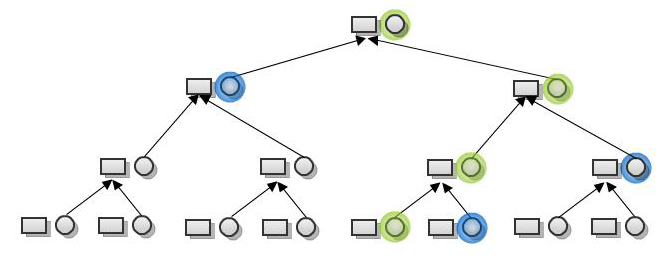
\includegraphics[width=100mm]{./images/8.jpg}
		\caption[]{Prover}
		\label{fig:proof}
		\end{figure}


\section{ Implementation }
\label{sec:impl}

	Implementing the SADS scheme was organized as follows.
	The first component to be implemented was the underlying data structure used by the prover and the mechanisms used by both prover and verifier to support the SADS scheme; mechanisms for determining a node's index in the tree and calculating partial digests for example.
	Then the data structures and mechanisms to support the query phase was added.
	Finally, these two parts were packaged as a library such that another project may leverage the scheme primitive and build applications on top of SADS.

	Our language of choice for this first stage of the project was Ruby.
	Ruby's main advantage was the ease of rapid prototyping as well as the vast collection of libraries available in the community.
	Specifically, the main component of the SADS scheme is the hash function which require matrix multiplication support.
	Ruby's standard library includes Vector and Matrix arithmetic operations which were sufficient for prototype scale implementations.
	Ruby was also a forward looking choice as we still have the option to create bindings for C and C++ code, when we require more efficient linear algebra libraries.

	The implementation in its current state as of this writing consists of two Ruby classes and one Ruby module.
	The classes are, not surprising, Prover and Verifier and the module is named Sads.
	Ruby has a feature called \textit{mixins} in which a module can be ``mixed into" a class.
	Mixing in a module has the effect of include all the module's fields and methods into the class definition.
	The Sads module contains any pieces of functionality required by both the Prover and the Verifier; the definition of the hash function for instance.
	However, since an instantiation of a Sads would not make sense, module mix-in was used instead of class inheritance.
	The Prover and Verifier classes then mix-in the functionality defined in Sads augmenting the Prover-only or Verifier-only functionality defined in their respective classes.
		Future iterations of this library will include a stronger focus on object-oriented design especially surrounding the nodes of the tree stored by the prover, the proofs generated per query requests, and abstractions surrounding the matrix multiplication so various linear algebra implementations can be swapped in and tested.

	The next stage was to implement the streaming setting in which the Prover and Verifier operate independently while witnessing a common stream of data.
	We wrote a very simple script to simulate such a scenario.
	This script was created as a new project, also using Ruby, and installed the SADS library via the RubyGems command `gem install --local $<$path to library$>$'.
	We wanted to ensure that the steps we took to use the SADS library in another project were the same as what we would expect other developers to do when using our library.
	The script takes three parameters to initialize the entire protocol, the security parameter, the upper bound on the size of the stream, and the size of the universe of stream elements.
	The Prover can be initialized from just these three parameter.
	The Verifier is then initialized with parameters provided to it from the Prover, similar to a client-server initialization wherein a client requests a session from a web server and can only proceed once the server grants the client the credentials.
	Finally in this small example, the user is then able to run commands such as ``add" which simulates the Prover and Verifier both witnessing some stream element or "query" which simulates a full membership query and response verification between Verifier to the Prover.

	The final stage is to implement the simulation across distributed computing infrastructure, that is, with a Prover and a Verifier which are not co-located.
	We imagine at least two possibilities for this implementation.
	One possibility could be a web service that plays matchmaker between ``needy" clients requesting prover services and ``generous" clients wishing to act as a prover.
	The web service would then facilitate communication between the two parties but would not provide the computational resources to act as either the prover or verifier.
	Another possibility, similar to the first, is one in which the web service itself acts as a Prover for any client requesting service.
	In either of these scenarios we imagine deploying a server application possibly built with EventMachine or Node.js or some other similar web application framework.
	Some proposed applications include monitoring and verifying of bandwidth charges from an ISP or continuous sensor data.

\section{Looking Forward}
\label{sec:forward}

	\subsection{ Benchmarking }

	The next stage of development is benchmarking to understand the performance of the implementation and to differentiate constraints resulting from particular design decisions from those arising from the schemes protocol itself.
	We will focus primarily on benchmarking the timing of important operations in the scheme as well as the memory footprint of the implementations largest data structures.

	We ran some preliminary calculations to ballpark the size of matrices \textbf{L} and \textbf{R}, the public key of the SADS scheme.
	Recall that \textbf{L} and \textbf{R} are matrices with elements in $Z_q$, that is elements are integers of at most $q$, which is itself derived from the security parameter, $k$ and the upper bound on the size of the stream, $n$.
	So a rough estimate of the size of \textbf{L} and \textbf{R} can be calculated by multiplying the dimensions of the matrices, by the amount of space required for each element.
	Below are two tables of estimations.

	\begin{table}[h]
	\centering

		\begin{tabular} { c | c | c | c}

		k & n & Matrix dim & Footprint\\ \hline
		1000&100000&1000 x 3000&14MB\\
		10000&100000&10000 x 30000&1716MB\\
		100000&100000&100000 x 300000&171661MB\\
		1000000&100000&1000000 x 3000000&20027160MB\\
		10000000&100000&10000000 x 30000000&2288818359MB\\
		\end{tabular}

	\caption{Estimation of public key size.  Constant stream size upper bound, varying security parameter }
	\label{tab:pub-key-k}
	\end{table}


	\begin{table}[h]
	\centering
		\begin{tabular}{ c | c | c | c}
		k & n & Matrix dim & Footprint\\ \hline
		500&10&500 x 1500&2MB\\
		500&100&500 x 1500&2MB\\
		500&1000&500 x 1500&2MB\\
		500&10000&500 x 1500&2MB\\
		500&100000&500 x 1500&3MB\\
		500&1000000&500 x 1500&3MB\\
		500&10000000&500 x 1500&4MB\\
		500&100000000&500 x 1500&4MB\\

		\end{tabular}
	\caption{ Estimation of public key size. Constant security parameter, varying stream size upper bound }
	\label{tab:pub-key-n}
	\end{table}


	The estimated memory footprint of the public key matrices grows rapidly with an increasing security parameter, but slowly with increasing stream size.
	The reason for this is that the scheme calls for matrices of size $k  \times ( k \times \log q )$.
	The matrix size grows faster than $k^2$ because $q$ also depends on $k$.
	Fortunately, the current proposal is to pick one security parameter which is large enough to provide the appropriate security properties for all instances of the SADS scheme.

	Future benchmarking efforts will also measure the memory footprint of the prover over time, and the size of a proof for varying parameter sizes. Additionally, we will benchmark the time required to perform the important updating and proof tasks for each of the prover and verifier.


	\subsection{ Production Quality Libraries }

	Through our benchmarking and profiling efforts, we hope to identify and fix the bottlenecks in implementation resulting in faster and higher quality code.
	We recognize that the built-in implementations of certain high cost operations, such as matrix multiplication may end up being the limiting factor, and as such we've identified a few options for future optimization.
	We hesitate to invest time and effort into any of these options too soon as we know that our first-draft implementation necessarily has room for improvement, but we outline those options here.

	\begin{enumerate}
	\item \textbf{SciRuby} : A Ruby library providing efficient implementations of linear algebra operations as well as other science, engineering, and visualization packages. \texttt{http://sciruby.com/}
	\item \textbf{NTL 5.5.2} : A free software written in C++ providing data structures and algorithms for arbitrary length integers, for vectors, matrices and polynomials over the integers and over the finite fields and for arbitrary precision floating point arithmetic. \texttt{http://shoup.net/ntl/}
	\item \textbf{MAGMA V2.18} : The kernel of Magma contains implementations of many of the important concrete classes of structure in five fundamental branches of algebra, namely group theory, ring theory, field theory, module theory and the theory of algebras.
	In addition, certain families of structures from algebraic geometry and finite incidence geometry are included. \texttt{http://magma.maths.usyd.edu.au/}
	\end{enumerate}


	%\subsection{Semester Outlook}
		%While the ultimate goal of the project is to produce a proof-of-concept application which utilizes a SADS scheme, it is best to set manage expectations.
		%Our baseline target for this semester is to complete the first two layers described above, that is the underlying data structure and the SADS scheme primitive.
		%Having completed these two components, we can then establish time line during which the proof-of-concept application can be hashed out and developed.
		%We hope to leverage the Ruby and broader open-source community by packaging this application, or just the SADS scheme primitive, into a library for others to use and provide feedback.


%%%%%%%%%%%%%%%%%%%%%%%%%%%%%%%%%%%%%%%%%%%%%%%%%%%%%%%%%%%%%%%%%%%%%%%%

\begin{thebibliography}{9}
	\bibitem{sads} Elaine Shi, Charalampos Papamanthou \emph{Streaming Authenticated Data Structures}, Date Unknown
%	\bibitem{evsc} B. Applebaum, Y. Ishai and E. Kushilevitz \emph{From Secrecy to Soundness: Efficient Verification via Secure Computation}
	\end{thebibliography}

\end{document}
